%!TEX root = ../thesis.tex
%*******************************************************************************
%*********************************** Results *********
%*******************************************************************************


\chapter{Results}

\ifpdf
    \graphicspath{{chapter-results/Figs/Raster/}{chapter-results/Figs/PDF/}{chapter-results/Figs/}}
\else
    \graphicspath{{chapter-results/Figs/Vector/}{chapter-results/Figs/}}
\fi

This chapter discusses the results of the different fit configurations and hypothesis tests performed in the analysis. After the background estimation obtained through a background-only fit in the \glspl{cr} is validated in the \glspl{vr}, the \glspl{sr} are unblinded and the observed data is compared to the \gls{sm} background expectation.

\section{Background-only fit results}\label{sec:results_background_only}

\subsection{Results in the control regions}

 \begin{figure}
	\centering
	\begin{subfigure}[b]{0.5\linewidth}
		\centering\includegraphics[width=0.85\textwidth]{OneLeptonbb_CR_TRLMEM_mct2_yellow}
	\end{subfigure}\hfill
	\begin{subfigure}[b]{0.5\linewidth}
		\centering\includegraphics[width=0.85\textwidth]{OneLeptonbb_CR_TRMMEM_mct2_yellow}
	\end{subfigure}\hfill
	\par\medskip
	\begin{subfigure}[b]{0.5\linewidth}
		\centering\includegraphics[width=0.85\textwidth]{OneLeptonbb_CR_TRHMEM_mct2_yellow}
	\end{subfigure}\hfill
	\begin{subfigure}[b]{0.5\linewidth}
		\centering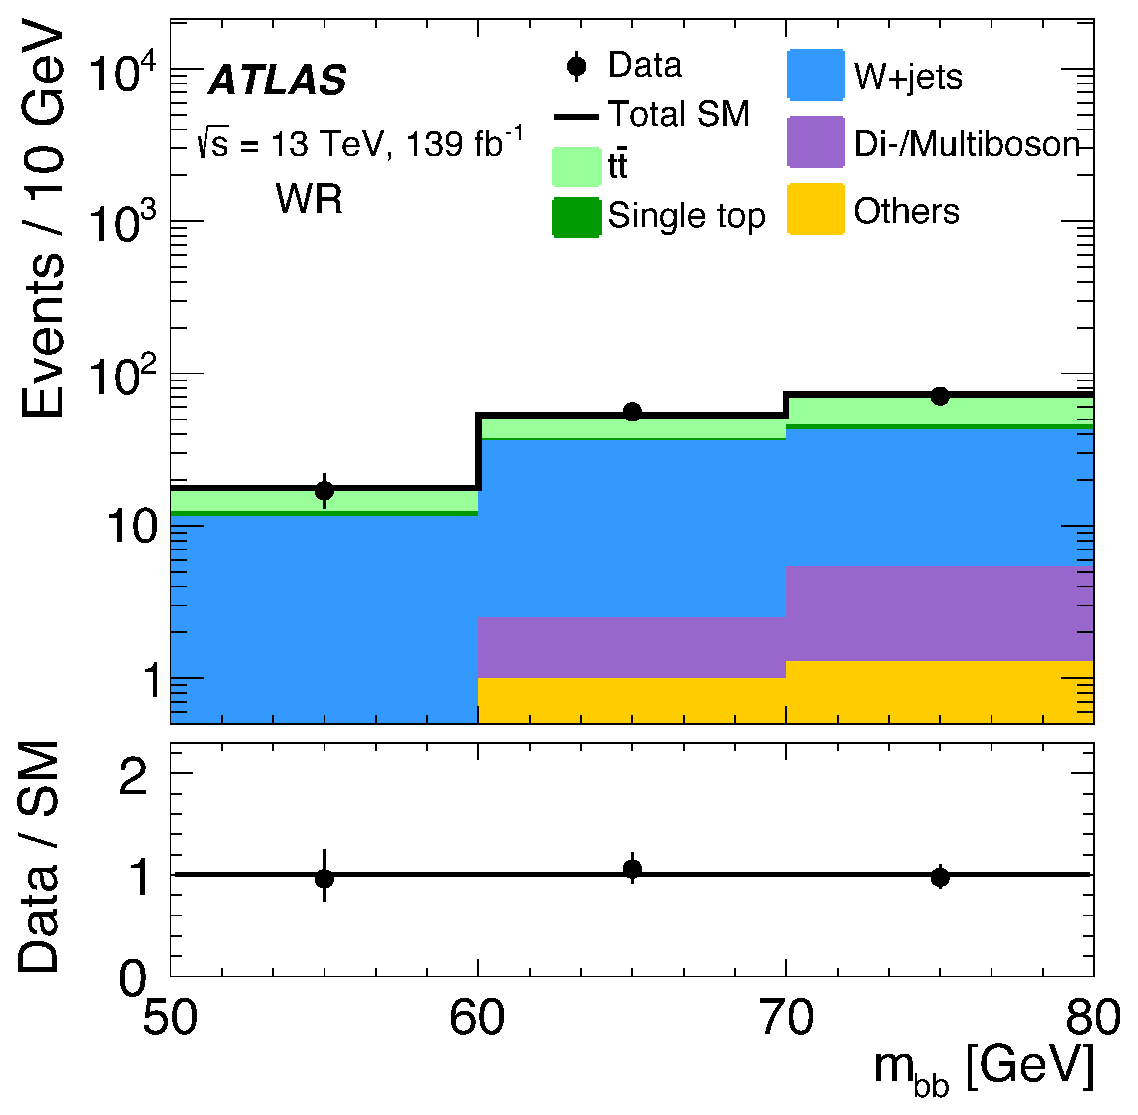
\includegraphics[width=0.85\textwidth]{OneLeptonbb_CR_WREM_mbb_yellow}
	\end{subfigure}\hfill
	\par\medskip
	\begin{subfigure}[b]{0.5\linewidth}
		\centering\includegraphics[width=0.85\textwidth]{OneLeptonbb_CR_STCREM_mbb_yellow}
	\end{subfigure}\hfill

	\caption{Exemplary distribution shown in each control region after the background-only fit. The shaded region includes all systematic uncertainties (including correlations) as well as \gls{mc} statistical uncertainty. The $\ttbar$, single top and $\wjets$ are normalised simultaneously in all \glspl{cr}. A good agreement between \gls{mc} expectation and data is observed in all \glspl{cr}.}
	\label{fig:CR_distributions_postfit}
\end{figure}



\begin{table}
\begin{center}
\setlength{\tabcolsep}{0.0pc}
{\small
%%
\begin{tabular*}{\textwidth}{@{\extracolsep{\fill}}lrrrrr}
\noalign{\smallskip}\hline\noalign{\smallskip}
{\textbf{ CR channel}}           & TRLM            & TRMM            & TRHM            & WR            & STCR              \\[-0.05cm]
\noalign{\smallskip}\hline\noalign{\smallskip}
%%
Observed events          & $657$              & $491$              & $641$              & $144$              & $155$                    \\
\noalign{\smallskip}\hline\noalign{\smallskip}
%%
Fitted bkg events         & $666 \pm 25$          & $480 \pm 21$          & $645 \pm 26$          & $143 \pm 12$          & $154 \pm 15$              \\
\noalign{\smallskip}\hline\noalign{\smallskip}
%%
        Fitted ttbar events         & $560 \pm 40$          & $430 \pm 33$          & $550 \pm 40$          & $47 \pm 9$          & $59 \pm 12$              \\
%%
        Fitted singletop events         & $60 \pm 40$          & $27 \pm 23$          & $33 \pm 27$          & $5 \pm 4$          & $57 \pm 22$              \\
%%
        Fitted wjets events         & $34 \pm 8$          & $10.5 \pm 2.8$          & $44 \pm 11$          & $83 \pm 16$          & $23 \pm 6$              \\
%%
        Fitted diboson events         & $4.3 \pm 1.2$          & $2.0 \pm 0.5$          & $2.8 \pm 0.5$          & $5.7 \pm 1.0$          & $2.8 \pm 0.9$              \\
%%
        Fitted $Z$+jets events         & $10.5 \pm 1.3$          & $10.6 \pm 1.4$          & $11.1 \pm 1.4$          & $2.4 \pm 0.4$          & $12.3 \pm 1.5$              \\
%%     
 \noalign{\smallskip}\hline\noalign{\smallskip}
%%
MC exp. SM events              & $720 \pm 80$          & $474 \pm 33$          & $680 \pm 50$          & $130 \pm 13$          & $180 \pm 50$              \\
\noalign{\smallskip}\hline\noalign{\smallskip}
%%
        MC exp. ttbar events         & $570 \pm 70$          & $407 \pm 30$          & $570 \pm 40$          & $46 \pm 10$          & $52 \pm 10$              \\
%%
        MC exp. singletop events         & $102 \pm 18$          & $46 \pm 13$          & $58 \pm 16$          & $9 \pm 6$          & $90 \pm 40$              \\
%%
        MC exp. wjets events         & $29 \pm 4$          & $8.4 \pm 1.2$          & $36.1 \pm 3.1$          & $67 \pm 5$          & $19.0 \pm 2.0$              \\
%%
        MC exp. diboson events         & $4.1 \pm 1.1$          & $2.0 \pm 0.5$          & $2.8 \pm 0.5$          & $5.6 \pm 1.0$          & $2.8 \pm 0.9$              \\
%%
        MC exp. $Z$+jets events         & $10.6 \pm 1.3$          & $10.6 \pm 1.4$          & $11.2 \pm 1.4$          & $2.5 \pm 0.4$          & $12.4 \pm 1.5$              \\
%%     \\
\noalign{\smallskip}\hline\noalign{\smallskip}
\end{tabular*}
%%%%
}
\end{center}
\caption{ Background fit results for the TRLMEM\_cuts, TRMMEM\_cuts, TRHMEM\_cuts, WREM\_cuts and STCREM\_cuts region(s),  for an integrated luminosity of $140.5$~\ifb.
%The results are obtained from the control regions using the discovery fit (see text for details). The fit results of the loose-not-tight regions are not shown.
Nominal MC expectations (normalised to MC cross-sections) are given for comparison. 
%The Monte Carlo QCD estimates are provided for illustrational purposes only, and are not used in the fit.
The errors shown are the statistical plus systematic uncertainties.
%, except for the error on the background estimate in the signal region, which is the systematic uncertainty only.
Uncertainties on the fitted yields are symmetric by construction, 
where the negative error is truncated when reaching to zero event yield.
}
\label{table.results.yields.fit.CR}
\end{table}
%

As all \glspl{cr} are mutually exclusive, a background-only fit simultaneously using information from all \glspl{cr} can be run. Only the terms for the \glspl{cr} enter the likelihood as channels and any signal contamination present in the \glspl{cr} is neglected. This allows to fit the dominant backgrounds to data, and thus by construction leads to a good agreement between observed data and the total fitted background estimate in all \glspl{cr}. The free normalisation parameters for $\ttbar$ ($\mu_\mathrm{T}$), single top ($\mu_\mathrm{ST}$) and $\wjets$ ($\mu_\mathrm{W}$) are fitted to be
\begin{equation}
	\begin{split}
		\mu_\mathrm{T} = 1.02^{+0.07}_{-0.09}, \\
		\mu_\mathrm{ST} = 0.6^{+0.5}_{-0.25}, \\
		\mu_\mathrm{W} = 1.22^{+0.26}_{-0.24}. \\
	\end{split}
\end{equation}
While the dominant $\ttbar$ background stays roughly at its nominal expectation with respect to \gls{mc} simulation, $\wjets$ processes are scaled up. The single top expectation, on the other hand, is scaled down. The high uncertainty on $\mu_\mathrm{ST}$ can be attributed to the relatively low \gls{mc} statistics as well as the comparably low purity of single top events in STR.

\Cref{tab:results_bkg_only_CR} summarises the fitted background estimate including all uncertainties for all control regions. As discussed in~\cref{ch:background_estimation}, $\ttbar$ is the most dominant in all control regions except WR where $\wjets$ is the largest background, followed by single top and $\wjets$ processes. Small contributions come from diboson, multiboson as well as other backgrounds like $\ttbar+V$, $\ttbar+h$ and $V+h$. All processes estimated directly from \gls{mc} simulation together account for only 10\%, 5.5\% and a maximum of 2.6\% in the single top, $\wjets$ and $\ttbar$ control regions, respectively. Exemplary distributions in the \glspl{cr} after the background-only fit are shown in~\cref{fig:VR_distributions_postfit}, revealing a good agreement between observed data and the \gls{sm} background estimate throughout the distributions shown.




\subsection{Results in the validation regions}



 \begin{figure}
	\centering
	\begin{subfigure}[b]{0.5\linewidth}
		\centering\includegraphics[width=0.85\textwidth]{OneLeptonbb_VR_UnderFlowBin_VRtt1offnomct2EM_mct2_yellow}
	\end{subfigure}\hfill
	\begin{subfigure}[b]{0.5\linewidth}
		\centering\includegraphics[width=0.85\textwidth]{OneLeptonbb_VR_UnderFlowBin_VRtt1onnomct2EM_mct2_yellow}
	\end{subfigure}\hfill
	\begin{subfigure}[b]{0.5\linewidth}
		\centering\includegraphics[width=0.85\textwidth]{OneLeptonbb_VR_UnderFlowBin_VRtt2offnomct2EM_mct2_yellow}
	\end{subfigure}\hfill
	\begin{subfigure}[b]{0.5\linewidth}
		\centering\includegraphics[width=0.85\textwidth]{OneLeptonbb_VR_UnderFlowBin_VRtt2onnomct2EM_mct2_yellow}
	\end{subfigure}\hfill
	\begin{subfigure}[b]{0.5\linewidth}
		\centering\includegraphics[width=0.85\textwidth]{OneLeptonbb_VR_UnderFlowBin_VRtt3offnomct2EM_mct2_yellow}
	\end{subfigure}\hfill
	\begin{subfigure}[b]{0.5\linewidth}
		\centering\includegraphics[width=0.85\textwidth]{OneLeptonbb_VR_UnderFlowBin_VRtt3onnomct2EM_mct2_yellow}
	\end{subfigure}\hfill

	\caption{Exemplary distributions shown in each validation region after the background-only fit with subsequent extrapolation to the \glspl{vr}. All selection cuts except for the requirement on $\mct$ (indicated using the red arrow) are applied. The shaded region includes all systematic uncertainties as well as \gls{mc} statistical uncertainty.}
	\label{fig:VR_distributions_postfit}
\end{figure}

\subsection{Results in the signal regions}


\begin{table}
\begin{center}
{\small
%%
\begin{tabular}{lrrrr}
\toprule
{\textbf{ SR-LM}}           & All $\mct$ bins          & Low $\mct$         & Medium $\mct$        & High $\mct$    \\[-0.05cm]
\midrule
Observed           & $34$              & $16$              & $11$              & $7$                    \\
\midrule
Expected          & $27 \pm 4~~$          & $8.8 \pm 2.8$          & $11.3 \pm 3.1~~$          & $7.3 \pm 1.5$              \\
\midrule
$\ttbar$          & $16.2 \pm 3.4~~$          & $4.4 \pm 2.2$          & $7.3 \pm 2.5$          & $4.6 \pm 1.2$              \\
Single top          & $2.7 \pm 1.8$          & $1.3 \pm 1.1$          & $0.9_{-0.9}^{+1.0}~$          & $0.6 \pm 0.6$              \\
$W$+jets           & $5.5 \pm 2.0$          & $2.0 \pm 0.9$          & $2.4 \pm 1.3$          & $1.1 \pm 0.5$              \\
Di-/Multiboson          & $0.67 \pm 0.19$          & $0.39 \pm 0.13$          & $0.09_{-0.09}^{+0.11}~$          & $0.18 \pm 0.04$              \\
Others          & $2.23 \pm 0.29$          & $0.81 \pm 0.25$          & $0.64 \pm 0.15$          & $0.77 \pm 0.12$              \\
\bottomrule
\textbf{ SR-MM}           & All $\mct$ bins          & Low $\mct$         & Medium $\mct$        & High $\mct$    \\[-0.05cm]
\midrule
Observed           & $13$              & $4$              & $7$              & $2$                    \\
\midrule
 Expected          & $8.6 \pm 2.2$          & $4.6 \pm 1.7$          & $2.6 \pm 1.3$          & $1.4 \pm 0.6$              \\
\midrule
$\ttbar$          & $2.7 \pm 1.4$          & $1.6 \pm 0.9$          & $0.8 \pm 0.7$          & $0.30 \pm 0.24$              \\
Single top          & $2.7 \pm 1.9$          & $1.6 \pm 1.5$          & $1.0_{-1.0}^{+1.1}~$          & $0.15_{-0.15}^{+0.19}~$              \\
$W$+jets          & $1.5 \pm 0.7$          & $0.6 \pm 0.4$          & $0.3_{-0.3}^{+0.4}~$          & $0.57 \pm 0.26$              \\
Di-/Multiboson          & $0.29 \pm 0.08$          & $0.09 \pm 0.04$          & $0.065 \pm 0.028$          & $0.14 \pm 0.06$              \\
Others          & $1.33 \pm 0.27$          & $0.69 \pm 0.20$          & $0.40 \pm 0.13$          & $0.24 \pm 0.09$              \\
\bottomrule
\textbf{ SR-HM}           & All $\mct$ bins          & Low $\mct$         & Medium $\mct$        & High $\mct$    \\[-0.05cm]
\midrule
Observed           & $14$              & $6$              & $5$              & $3$                    \\
\midrule
 Expected          & $8.1 \pm 2.7$          & $4.1 \pm 1.9$          & $2.9 \pm 1.3$          & $1.1 \pm 0.5$              \\
\midrule
         $\ttbar$          & $1.4 \pm 0.5$          & $0.8 \pm 0.4$          & $0.36 \pm 0.25$          & $0.22 \pm 0.15$              \\
Single top          & $2.0_{-2.0}^{+2.4}~$          & $0.9_{-0.9}^{+1.5}~$         & $0.9 \pm 0.9$          & $0.16_{-0.16}^{+0.26}~$              \\
$W$+jets           & $3.7 \pm 1.0$          & $1.9 \pm 0.8$          & $1.4 \pm 0.8$          & $0.45 \pm 0.19$              \\
Di-/Multiboson          & $0.21 \pm 0.06$          & $0.057 \pm 0.025$          & $0.075 \pm 0.027$          & $0.08 \pm 0.04$              \\
Others          & $0.74 \pm 0.16$          & $0.34 \pm 0.09$          & $0.19 \pm 0.08$          & $0.21 \pm 0.08$              \\
\bottomrule
\end{tabular}
}
\end{center}
\caption{ Background-only fit results in the exclusion \glspl{sr} for an integrated luminosity of \onethirtynineifb. The first column shows the sum of all $\mct$ bins (including overflow). Subsequent columns indicate the different bins in $\mct$, overflow is included in the last bin. The errors shown include the \gls{mc} statistical and systematic uncertainties. Uncertainties in the fitted yields are symmetric by construction, except where the negative error is truncated at an event yield of zero. PDG rounding is applied to the event rates and uncertainties~\cite{pdg2020}. Table adapted from \reference\cite{SUSY-2019-08}.}\label{tab:results_bkg_only_SR}
\end{table}
%


 \begin{figure}
	\centering
	\begin{subfigure}[b]{0.5\linewidth}
		\centering\includegraphics[width=0.85\textwidth]{OneLepton_Wh_SRLMEM_mct2_yellow}
	\end{subfigure}\hfill
	\begin{subfigure}[b]{0.5\linewidth}
		\centering\includegraphics[width=0.85\textwidth]{OneLepton_Wh_SRMMEM_mct2_yellow}
	\end{subfigure}\hfill
	\begin{subfigure}[b]{0.5\linewidth}
		\centering\includegraphics[width=0.85\textwidth]{OneLepton_Wh_SRHMEM_mct2_yellow}
	\end{subfigure}\hfill

	\caption{Exemplary distribution shown in each exclusion signal region after the background-only fit. The shaded region includes all systematic uncertainties (including correlations) as well as \gls{mc} statistical uncertainty.}
	\label{fig:SR_distributions_postfit}
\end{figure}

\section{Interpretation}

 \begin{figure}
	\centering\includegraphics[width=0.85\textwidth]{histpull_CRVRSR}
	\caption{}
	\label{fig:result_exclusion}
\end{figure}



\begin{table}
\begin{center}
%\resizebox{\textwidth}{!}{
\begin{tabular}{lcccccc}
\toprule
\textbf{Signal Region}                       & $\langle\epsilon{\mathrm{ \sigma}}\rangle_{\mathrm{ obs}}^{95}$[fb]  &  $S_{\mathrm{ obs}}^{95}$  & $S_{\mathrm{ exp}}^{95}$ & $\textrm{CL}_{\textrm{B}}$ & $p_{0}$ & $Z$  \\
\midrule
 SRLM $\mathrm{(disc.)}$    & $0.26$ &  $36.8$ & $ { 20.0 }^{ +8.0 }_{ -5.4 }$ & $0.97$ & $ 0.03$&$1.88$ \\%
 SRMM $\mathrm{(disc.)}$    & $0.18$ &  $24.8$ & $ { 15.3 }^{ +6.2 }_{ -4.6 }$ & $0.94$ & $ 0.06$&$1.54$ \\%
 SRHM $\mathrm{(disc.)}$    & $0.11$ &  $14.7$ & $ { ~~9.7 }^{ +3.3 }_{ -2.7 }$ & $0.89$ & $ 0.10$&$1.30$ \\%

\bottomrule
\end{tabular}
%}
\caption[Breakdown of upper limits.]{
Left to right: 95\% CL upper limits on the visible cross-section
($\langle\epsilon\sigma\rangle_{\mathrm{ obs}}^{95}$) and on the number of
signal events ($S_{\mathrm{ obs}}^{95}$ ). 
The third column ($S_{\mathrm{ exp}}^{95}$) shows the expected 95\% CL upper limit (and its $\pm 1\sigma$ excursions) 
on the number of signal events if no BSM signal is present. 
% on the number of signal events that would be expected were the observation consistent with a background-only hypothesis, (and $\pm 1\sigma$ excursions on the expectation) of background events.
The last three columns
indicate the $\textrm{CL}_{\textrm{B}}$ value, i.e. the confidence level observed for
the background-only hypothesis, the discovery $p$-value ($p_{0}$) and the significance $Z$~\cite{2008NIMPA.595..480C}.}
\label{upperlimit_toys}
\end{center}
\end{table}


 \begin{figure}
	\centering\includegraphics[width=0.75\textwidth]{contourPlotterWh1Lbb}
	\caption{}
	\label{fig:result_exclusion}
\end{figure}




